% Source: http://www.brian-amberg.de/uni/poster/
\documentclass[landscape,archE,fontscale=0.2]{baposter}
\usepackage[vlined]{algorithm2e}
\usepackage{times,calc}
\usepackage{amsmath,amssymb}
\usepackage{relsize}
\usepackage{multirow,multicol}
\usepackage{ae}
\usepackage{url}

\usepackage[T1]{fontenc}
\renewcommand{\familydefault}{\sfdefault}

\usepackage{enumitem}\setlist{nolistsep,leftmargin=*}
\usepackage{graphicx}\graphicspath{{images/}}

\usepackage{tikz}
\usetikzlibrary[topaths]
\newcount\mycount

\usepackage[
citestyle=numeric,
firstinits=true,
maxcitenames=1,
]{biblatex}
\bibliography{refs}

\setlength{\columnsep}{0.7em}\setlength{\columnseprule}{0mm}

\definecolor{crimsonRed}{cmyk}{0, 1, 1, 0.4}

\begin{document}
\begin{poster}{
    grid=false,
    colspacing=0.7em,
    headerColorOne=crimsonRed, borderColor=crimsonRed,
    textborder=faded,
    headerborder=open, headershape=roundedright,
    headershade=plain, headerFontColor=white,
    background=none, bgColorOne=white,
    headerheight=0.15\textheight,
    headerfont=\color{white}\textsf\textbf\Large,
    columns=3
  }{
    
\includegraphics[height=0.13\textheight]{cmu-seal}
  }{
    {\textsc{\textbf{\LARGE Title}}} \\
    {\Large Subtitle}
  }{\vspace{2mm}\large
    Brandon Amos and $\ldots$ \\
    School of Computer Science,
    Carnegie Mellon University
  }{
    
\includegraphics[height=0.11\textheight]{cmu-logo}
  }

  \headerbox{Introduction and Background}
  {name=intro,column=0,row=0}{\begin{itemize}
\item Item 1\cite{article}
\item Item 2
\item Item 3
\end{itemize}}

  \headerbox{Design}
  {name=design,column=1,row=0}{\begin{center}
  % http://www.texample.net/tikz/examples/complete-graph/
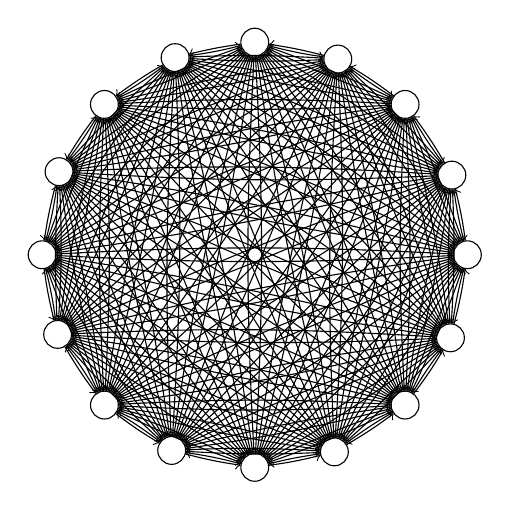
\begin{tikzpicture}[transform shape, scale=0.5]
  %the multiplication with floats is not possible. Thus I split the loop in two.
  \foreach \number in {1,...,8}{
      % Computer angle:
        \mycount=\number
        \advance\mycount by -1
  \multiply\mycount by 45
        \advance\mycount by 0
      \node[draw,circle,inner sep=0.25cm] (N-\number) at (\the\mycount:5.4cm) {};
    }
  \foreach \number in {9,...,16}{
      % Computer angle:
        \mycount=\number
        \advance\mycount by -1
  \multiply\mycount by 45
        \advance\mycount by 22.5
      \node[draw,circle,inner sep=0.25cm] (N-\number) at (\the\mycount:5.4cm) {};
    }
  \foreach \number in {1,...,15}{
        \mycount=\number
        \advance\mycount by 1
  \foreach \numbera in {\the\mycount,...,16}{
    \path (N-\number) edge[->,bend right=3] (N-\numbera)  edge[<-,bend
      left=3] (N-\numbera);
  }
}
\end{tikzpicture}
  % http://www.texample.net/tikz/examples/complete-graph/
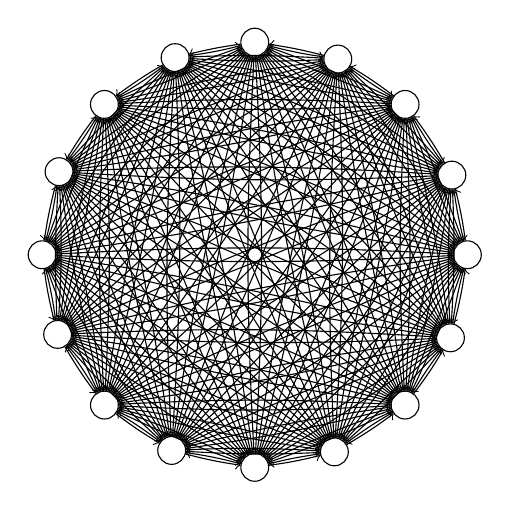
\begin{tikzpicture}[transform shape, scale=0.5]
  %the multiplication with floats is not possible. Thus I split the loop in two.
  \foreach \number in {1,...,8}{
      % Computer angle:
        \mycount=\number
        \advance\mycount by -1
  \multiply\mycount by 45
        \advance\mycount by 0
      \node[draw,circle,inner sep=0.25cm] (N-\number) at (\the\mycount:5.4cm) {};
    }
  \foreach \number in {9,...,16}{
      % Computer angle:
        \mycount=\number
        \advance\mycount by -1
  \multiply\mycount by 45
        \advance\mycount by 22.5
      \node[draw,circle,inner sep=0.25cm] (N-\number) at (\the\mycount:5.4cm) {};
    }
  \foreach \number in {1,...,15}{
        \mycount=\number
        \advance\mycount by 1
  \foreach \numbera in {\the\mycount,...,16}{
    \path (N-\number) edge[->,bend right=3] (N-\numbera)  edge[<-,bend
      left=3] (N-\numbera);
  }
}
\end{tikzpicture}
\end{center}}

  \headerbox{Results}
  {name=results,column=2}{\begin{center}
  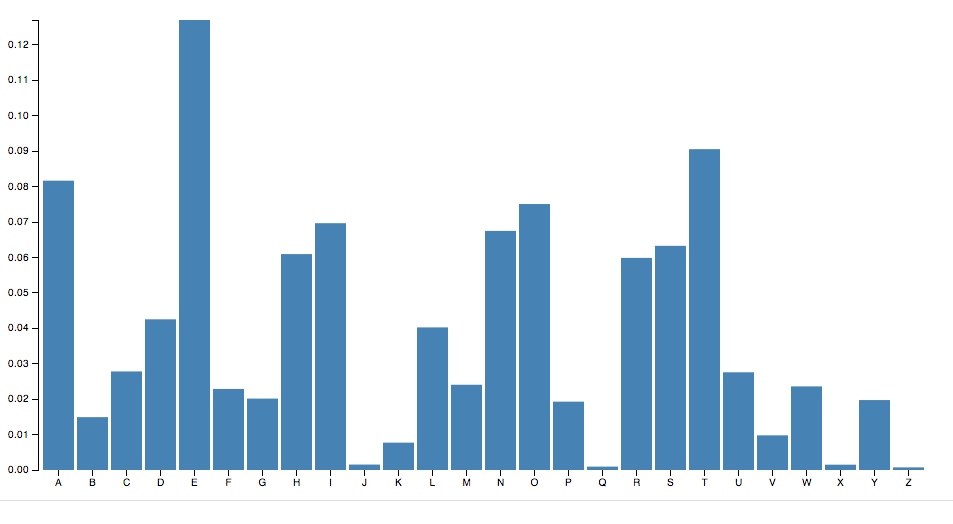
\includegraphics[width=\textwidth]{results}
  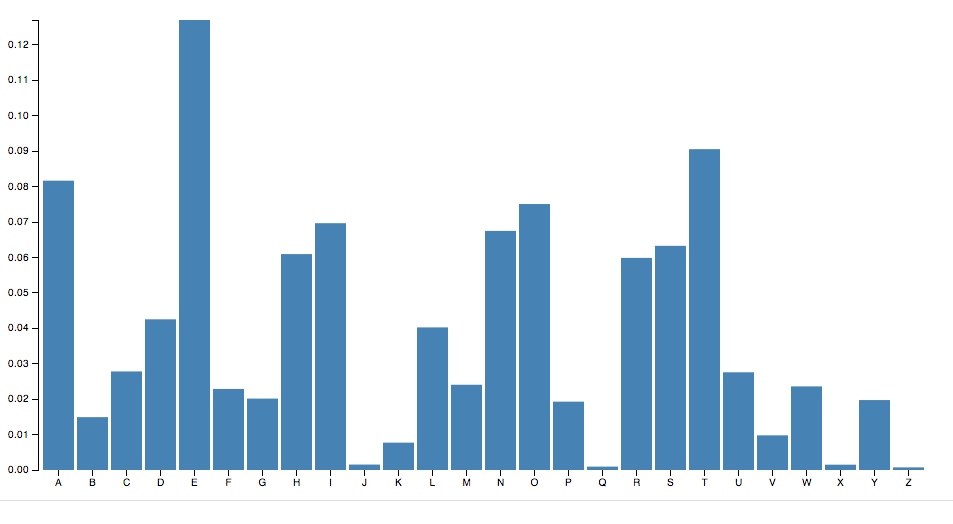
\includegraphics[width=\textwidth]{results}
\end{center}}

  % Below lowest section.
  \headerbox{References}
  {name=refs,column=0,below=design,above=bottom,span=3}{
    \setlength{\bibitemsep}{0pt}
    \renewcommand*{\bibfont}{\footnotesize}
    \printbibliography[heading=none]
  }

  % Sections bordering references that aren't the lowest.
  \headerbox{Contributions}
  {name=contrib,column=0,below=intro,above=refs}{\begin{itemize}
\item Item 1
\item Item 2
\item Item 3
\item Item 4
\end{itemize}}

  \headerbox{Conclusions}
  {name=conclusions,column=2,below=results,above=refs}{\begin{itemize}
\item Item 1
\item Item 2
\item Item 3
\item Item 4
\end{itemize}}

\end{poster}
\end{document}
